% Memoria de la fase 1 del proyecto 1 de PIDS 26/27: reconocimiento de gestos de mano.
% Compilar desde esta carpeta:  latexmk -pdf informe_fase1.tex
% Las figuras salen de ../resultados (las mismas que enlazan los informes de cada experimento).
\documentclass[11pt,a4paper]{article}

\usepackage[utf8]{inputenc}
\usepackage[T1]{fontenc}
\usepackage[spanish,es-tabla,es-noshorthands]{babel}
\usepackage{lmodern}
\usepackage{microtype}
\usepackage[margin=2.4cm]{geometry}
\usepackage{amsmath}
\usepackage{siunitx}
\sisetup{group-separator={\,},group-minimum-digits=5,output-decimal-marker={,}}
\usepackage{graphicx}
\usepackage{booktabs}
\usepackage{tabularx}
\usepackage{multirow}
\usepackage{float}
\usepackage{caption}
\usepackage{subcaption}
\usepackage{enumitem}
\usepackage[table]{xcolor}
\usepackage{tikz}
\usetikzlibrary{arrows.meta,positioning}
\usepackage{fancyhdr}
\usepackage{titlesec}
\usepackage[hidelinks]{hyperref}

\definecolor{azul}{HTML}{2563EB}
\definecolor{tinta}{HTML}{1E3A8A}
\definecolor{gris}{HTML}{64748B}
\definecolor{fondo}{HTML}{EEF4FF}

\graphicspath{{../resultados/principal/figuras/}{../resultados/clustering/}}
\captionsetup{font=small,labelfont={bf,color=tinta}}
\titleformat{\section}{\Large\bfseries\color{tinta}}{\thesection}{0.8em}{}
\titleformat{\subsection}{\large\bfseries\color{tinta}}{\thesubsection}{0.8em}{}
\setlist{itemsep=2pt,topsep=4pt}
\setlength{\parskip}{4pt}
\setlength{\emergencystretch}{3em}

\pagestyle{fancy}
\fancyhf{}
\fancyhead[L]{\small\color{gris}PIDS 26/27 · Proyecto 1 · Fase 1}
\fancyhead[R]{\small\color{gris}Reconocimiento de gestos de mano}
\fancyfoot[C]{\small\thepage}
\renewcommand{\headrulewidth}{0.4pt}

\newcommand{\pct}[1]{#1\,\%}
\newcommand{\codigo}[1]{\texttt{#1}}
\newcommand{\mejor}[1]{\textbf{#1}}

\begin{document}

% ------------------------------------------------------------------ portada
\begin{titlepage}
  \centering
  \vspace*{2.5cm}
  {\large\color{gris} PIDS 26/27 · Proyecto 1 · Fase 1\par}
  \vspace{1.2cm}
  {\Huge\bfseries\color{tinta} Reconocimiento de gestos de mano\par}
  \vspace{0.5cm}
  {\Large Del dataset grabado por el grupo al modelo que se ejecuta en el navegador\par}
  \vspace{2cm}
  \begin{tikzpicture}[caja/.style={draw=azul,fill=fondo,rounded corners=3pt,minimum height=1cm,minimum width=2.35cm,align=center,font=\small},
                      flecha/.style={-{Latex[length=2.2mm]},thick,azul}]
    \node[caja] (a) {Cámara};
    \node[caja,right=0.45cm of a] (b) {MediaPipe\\21 puntos};
    \node[caja,right=0.45cm of b] (c) {Normalización};
    \node[caja,right=0.45cm of c] (d) {MLP\\6 gestos};
    \draw[flecha] (a) -- (b); \draw[flecha] (b) -- (c); \draw[flecha] (c) -- (d);
  \end{tikzpicture}
  \vfill
  {\large Javier Saguar · Alejandro Cuevas · Mónica Fernández\\[2pt] Pedro José Orrego · Daniel Naval\par}
  \vspace{0.8cm}
  {\color{gris} Universidad Politécnica de Madrid · ETSI de Telecomunicación\\ Octubre de 2026\par}
\end{titlepage}

\begin{abstract}
\noindent Esta memoria describe la primera fase del proyecto: un reconocedor de seis gestos de mano a partir de la
cámara de un portátil. Grabamos un dataset propio de \num{3000} imágenes con cinco personas, extrajimos los 21 puntos
de la mano con MediaPipe y comparamos siete familias de modelos con cuatro normalizaciones geométricas. Para medir de
forma honesta evaluamos siempre con una persona que el modelo no ha visto (\emph{leave-one-participant-out}, LOPO).
La normalización respecto a la muñeca, la escala y el giro es la decisión que más influye: sube la CNN del
enunciado del \pct{90,9} al \pct{95,8}. El modelo elegido es un perceptrón multicapa (MLP) de \num{5030}
parámetros que alcanza un \pct{96,5} en LOPO, ocupa 86~KB y clasifica en 0,84~ms; se exporta a JSON y se ejecuta en el
navegador con las mismas probabilidades que en Python. Un análisis sin etiquetas confirma que la normalización ya
separa los gestos, aunque cada uno está formado por varias variantes que solo un clasificador supervisado une.
\end{abstract}

\tableofcontents
\newpage

% ------------------------------------------------------------------ 1
\section{Objetivo}

El enunciado pide reconocer gestos de mano con MediaPipe y un clasificador entrenado sobre un dataset grabado por el
grupo, y usarlos para dar órdenes. Nos fijamos tres objetivos:

\begin{enumerate}
  \item \textbf{Un dataset propio y variado}, con varias personas, distancias, ángulos y posiciones, grabado de forma
        que se pueda evaluar con personas nuevas.
  \item \textbf{Una evaluación honesta}: medir el acierto con alguien a quien el modelo no ha visto nunca, que es lo que
        ocurre en una demostración.
  \item \textbf{Un modelo ligero}, capaz de funcionar en tiempo real en el portátil y también en el navegador, para
        integrarlo después con la plataforma de datos y los chatbots (fases 2 y 3) sin enviar ninguna imagen.
\end{enumerate}

% ------------------------------------------------------------------ 2
\section{Grabación del dataset}

\subsection{Los seis gestos}

Elegimos seis gestos fáciles de hacer y de explicar. Cada uno tiene asignada una orden del vehículo tanque del
enunciado (en el portal web de la fase 2 tienen otras acciones, como cambiar de sección o abrir el asistente).

\begin{table}[H]
\centering\small
\begin{tabularx}{\linewidth}{llX l}
\toprule
Clase & Gesto & Cómo se hace & Orden del tanque \\
\midrule
\codigo{ok} & OK & Pulgar e índice en círculo; los otros tres dedos extendidos y separados & GIRAR \\
\codigo{paper} & Papel & Mano abierta, dedos extendidos y separados, palma hacia la cámara & PARAR \\
\codigo{rock} & Piedra & Puño cerrado con el pulgar recogido por delante & RETROCEDER \\
\codigo{rockandroll} & Cuernos & Índice y meñique extendidos; corazón y anular doblados & DISPARAR \\
\codigo{scissors} & Tijera & Índice y corazón en V bien abierta; el resto cerrado & HACER FOTO \\
\codigo{thumbsup} & Pulgar arriba & Puño con el pulgar extendido hacia arriba & AVANZAR \\
\bottomrule
\end{tabularx}
\caption{Gestos del dataset.}
\end{table}

Dos pares se parecen mucho y la guía de grabación los destacaba: \codigo{rock} y \codigo{thumbsup}, que solo se
diferencian en el pulgar, y \codigo{scissors} y \codigo{rockandroll}. Como se verá en la sección~\ref{sec:resultados},
son precisamente los que más se confunden.

\subsection{Kit de grabación}

Partimos del grabador del repositorio de la asignatura (\codigo{efhes/IE-workspace}) y lo adaptamos para que cada
persona grabara en Windows con la webcam de su portátil, sin Raspberry Pi. El kit (\codigo{kit\_grabacion/}) se instala
con Python~3.12 y funciona así:

\begin{itemize}
  \item Al arrancar pide un \textbf{identificador de participante} (\codigo{p1} a \codigo{p5}) y la mano con la que se
        va a grabar. El identificador es la base de la evaluación por persona, así que cada uno usa siempre el suyo.
  \item Para cada gesto, la ventana muestra los puntos detectados por MediaPipe; solo cuando se ven se pulsa
        \codigo{s} y empieza la captura: \textbf{una imagen por segundo durante 100 segundos}.
  \item Cada toma se guarda en una carpeta nueva con fecha y hora y un \codigo{metadata.json} con su estado
        (completa, interrumpida o en curso), de modo que ninguna grabación se pisa.
  \item Un modo de prueba graba 5 imágenes por gesto en otra carpeta para comprobar cámara, luz y detección.
\end{itemize}

\subsection{Reglas de calidad}

Si la persona se queda quieta, las 100 imágenes de un gesto son casi el mismo fotograma y el modelo memoriza una
postura. Por eso la guía pedía moverse despacio y de forma continua durante los 100 segundos: acercarse a unos 30~cm
y alejarse hasta 1~m, girar e inclinar la muñeca y recorrer el encuadre, siempre con la misma mano.

\subsection{Resultado de la grabación}

Cinco personas grabaron una toma completa cada una: 6 gestos $\times$ 100 imágenes $\times$ 5 personas =
\textbf{\num{3000} imágenes}. Otras cuatro tomas quedaron interrumpidas o vacías (0, 6, 0 y 0 imágenes) y se descartan
automáticamente por su estado. MediaPipe detecta la mano en \textbf{\num{2931} imágenes (\pct{97,7})}; las imágenes
sin mano no se usan.

\begin{table}[H]
\centering\small
\begin{tabular}{lrrrcc}
\toprule
Participante & Imágenes & Con mano & Detección & Tamaño de la mano (p5--p95) & Máx./mín. \\
\midrule
p1 & 600 & 572 & \pct{95,3} & 0,10 -- 0,26 & 2,5$\times$ \\
p2 & 600 & 585 & \pct{97,5} & 0,14 -- 0,41 & 2,9$\times$ \\
p3 & 600 & 588 & \pct{98,0} & 0,17 -- 0,29 & 1,7$\times$ \\
p4 & 600 & 599 & \pct{99,8} & 0,16 -- 0,30 & 1,9$\times$ \\
p5 & 600 & 587 & \pct{97,8} & 0,11 -- 0,24 & 2,1$\times$ \\
\bottomrule
\end{tabular}
\caption{Tomas válidas. El tamaño de la mano es la distancia de la muñeca al nudillo del corazón, en unidades de alto
de imagen: cuanto mayor, más cerca de la cámara.}
\label{tab:dataset}
\end{table}

La figura~\ref{fig:diversidad} confirma que la grabación es variada: el tamaño de la mano cambia entre 1,7 y 2,9 veces
dentro de cada toma y la inclinación respecto a la vertical recorre unos $\pm 70^\circ$. La detección más baja es la de
\codigo{rock} (\pct{89} en p5 y \pct{92} en p1): con el puño cerrado hay menos dedos visibles.

\begin{figure}[H]
\centering
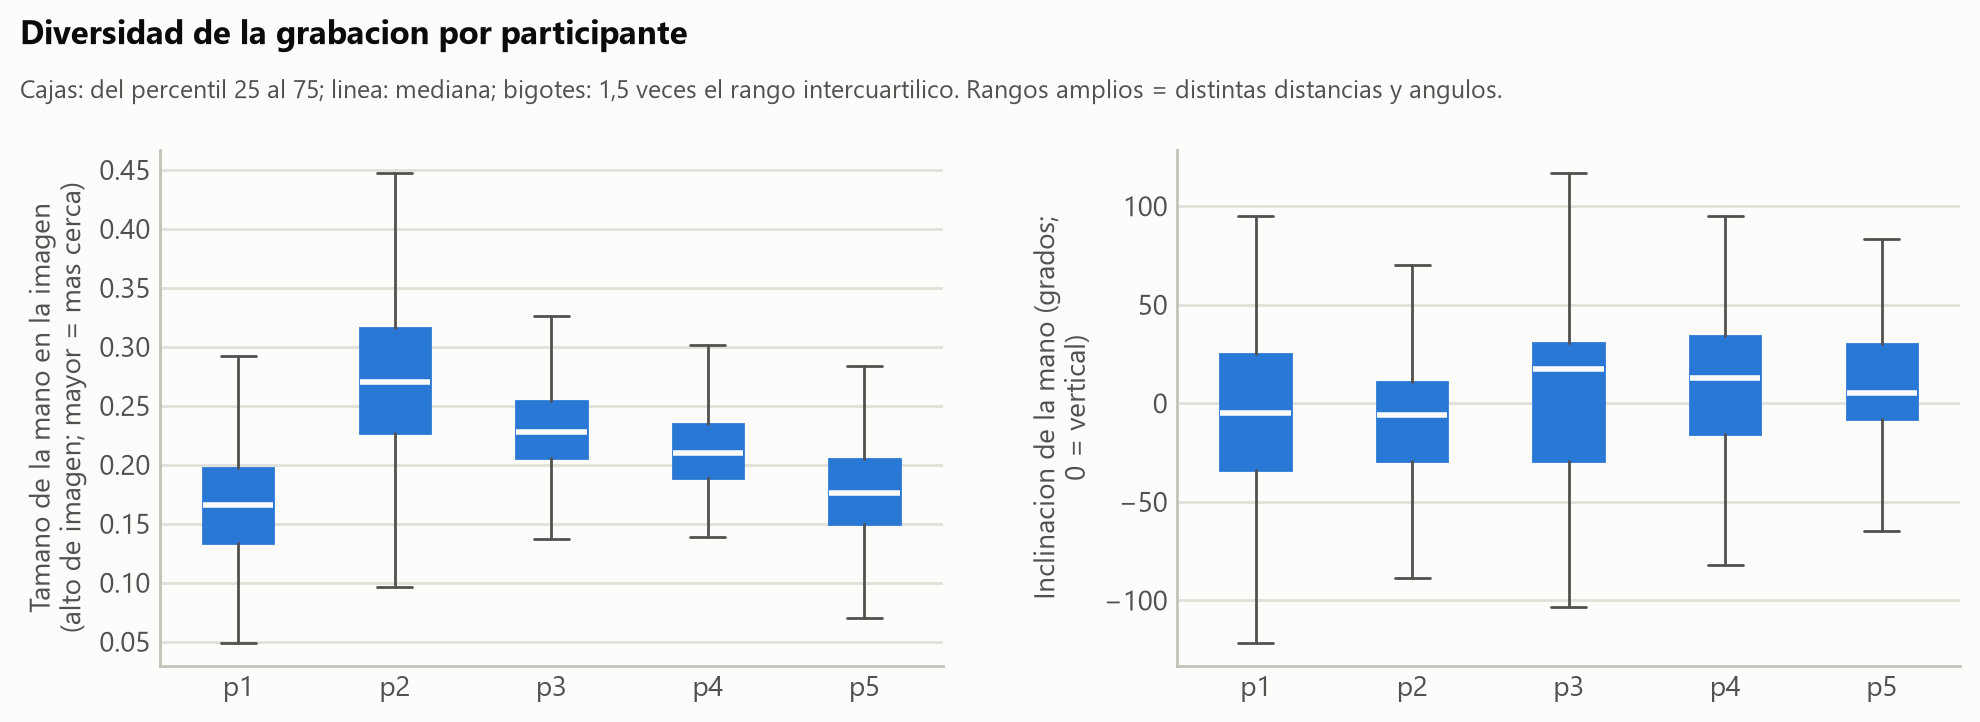
\includegraphics[width=\linewidth]{diversidad_dataset}
\caption{Diversidad de distancias (izquierda) y de inclinaciones (derecha) por participante.}
\label{fig:diversidad}
\end{figure}

La etiqueta de mano izquierda o derecha que devuelve MediaPipe no es fiable en este dataset: ronda el \pct{50} en todas
las tomas aunque cada persona grabó con una sola mano, porque al girar la muñeca el dorso de una mano tiene en 2D la
misma forma que la palma de la otra.

\subsection{Privacidad y copia de seguridad}

Las imágenes muestran la cara de los cinco integrantes, así que \textbf{no se publican} en el repositorio, que es
público. Se guardan en una copia comprimida y verificada (\codigo{dataset\_gestos\_PIDS\_2026-09-16.zip}, 599~MB,
con el SHA-256 de cada fichero) que se comparte solo con el grupo y los profesores. Por el mismo motivo, la figura de
errores con fotos que genera el pipeline tampoco se publica. En el repositorio están los puntos de la mano extraídos
(\codigo{datos\_generados/}), que es todo lo que necesitan los modelos.

% ------------------------------------------------------------------ 3
\section{De la imagen a la representación}

\subsection{Puntos de la mano en vez de píxeles}

MediaPipe Hands localiza 21 puntos de la mano (muñeca, nudillos y articulaciones de cada dedo). Clasificamos esas
coordenadas y no la imagen por tres motivos:

\begin{itemize}
  \item \textbf{Generaliza mejor}: los puntos no dependen del fondo, la luz, la ropa ni el tono de piel, de modo que el
        modelo aprende la forma de la mano y no el entorno de quien grabó.
  \item \textbf{Es pequeño}: 42 números por mano ($x$, $y$ de 21 puntos) frente a cientos de miles de píxeles.
  \item \textbf{No cuesta tiempo}: MediaPipe tarda 16,1~ms por fotograma de $1280\times720$, y eso ya fija el ritmo; el
        clasificador añade menos de 1~ms (sección~\ref{sec:coste}).
\end{itemize}

\subsection{Corrección del aspecto}

MediaPipe devuelve $x$ dividida por el ancho de la imagen e $y$ dividida por el alto. En una imagen de
$1280\times720$, una unidad de $x$ mide 1,78 veces lo que una de $y$, así que medir distancias o girar sobre esas
coordenadas deforma la mano. Antes de nada se pasa a un espacio con el aspecto corregido:
\[
  \tilde{x}_i = x_i \cdot \frac{\text{ancho}}{\text{alto}}, \qquad \tilde{y}_i = y_i, \qquad i = 0, \dots, 20 .
\]

\subsection{Normalizaciones}

Probamos cuatro representaciones, cada una añadiendo un paso a la anterior. Sea $\mathbf{p}_i$ el punto $i$ con el
aspecto corregido, $\mathbf{p}_0$ la muñeca y $\mathbf{p}_9$ el nudillo del dedo corazón:

\begin{enumerate}
  \item \textbf{Ninguna}: las coordenadas de MediaPipe tal cual, como hace el notebook de la asignatura. La posición de
        la mano en el encuadre pasa a ser un dato más, aunque no debería influir en el gesto.
  \item \textbf{Muñeca}: $\mathbf{q}_i = \mathbf{p}_i - \mathbf{p}_0$. Quita la posición en el encuadre.
  \item \textbf{Muñeca + escala}: $\mathbf{q}_i = (\mathbf{p}_i - \mathbf{p}_0)/s$, con
        $s = \lVert \mathbf{p}_9 - \mathbf{p}_0 \rVert$. Esa distancia apenas cambia entre gestos porque la palma no se
        deforma, así que quita la dependencia de la distancia a la cámara.
  \item \textbf{Muñeca + escala + giro}: además se gira la mano para que el vector muñeca--nudillo del corazón apunte
        siempre hacia arriba. Quita la inclinación. A cambio, dos gestos que solo se distinguieran por su orientación
        (pulgar arriba y pulgar abajo) dejarían de poder separarse; entre nuestros seis gestos no ocurre.
\end{enumerate}

\subsection{Invarianza a la mano y aumentación}

Cada persona grabó con una mano, pero en la demo se puede usar cualquiera. Probamos dos estrategias alternativas:

\begin{itemize}
  \item \textbf{Espejo}: reflejar las manos que MediaPipe etiqueta como izquierdas para llevarlas todas a la misma
        lateralidad. Depende de una etiqueta que, como vimos, no es fiable.
  \item \textbf{Aumentación con volteo}: añadir al entrenamiento copias perturbadas de cada mano (giro aleatorio de
        hasta $\pm15^\circ$, escala de $\pm$\pct{10}, desplazamiento de hasta 0,05 y ruido gaussiano en cada punto,
        que imita el temblor de MediaPipe) y voltear horizontalmente la mitad. El modelo aprende las dos manos solo con
        datos.
\end{itemize}

La misma cadena de transformaciones se aplica al entrenar, en la demo de Windows y en el navegador.

% ------------------------------------------------------------------ 4
\section{Modelos}

Comparamos siete familias. Cada una responde a una pregunta distinta sobre el problema:

\begin{table}[H]
\centering\small
\begin{tabularx}{\linewidth}{lX}
\toprule
Modelo & Arquitectura y motivo \\
\midrule
CNN del enunciado & Entrada $21\times2$; dos capas Conv2D de 16 filtros con núcleo que recorre 5 puntos, ReLU, Dense(32) y
softmax. Es la referencia que pide el enunciado. \\
CNN del notebook & La que construye de verdad el notebook de la asignatura: una sola Conv2D y \emph{dropout} de 0,3.
Se entrena en el propio notebook, como comprobación. \\
MLP & Perceptrón multicapa $42 \rightarrow 64 \rightarrow 32 \rightarrow 6$ con \emph{dropout} de 0,2. Pregunta: si la
entrada ya es geometría, ¿hacen falta convoluciones? \\
SVM & Núcleo RBF ($C=10$) sobre las coordenadas estandarizadas. Fuerte con pocos datos y pocas dimensiones. \\
Random forest & 200 árboles. No lineal y sin necesidad de escalar; grande en disco. \\
Regresión logística & Base lineal: ¿basta una frontera recta tras normalizar? \\
$k$ vecinos & $k=5$, sin entrenamiento: clasifica por las 5 manos más parecidas del entrenamiento. Cota inferior sencilla. \\
\bottomrule
\end{tabularx}
\caption{Modelos comparados.}
\end{table}

Las redes usan los hiperparámetros del notebook (AdamW con tasa 0,001, \emph{weight decay} de $10^{-4}$, lotes de 32
y parada temprana sobre la pérdida de validación) con una diferencia: hasta 200 épocas con paciencia 20 en lugar de 300
y 50, porque la mejor época llegaba de media en la 23 en LOPO. Todo se entrenó con Keras~3 sobre PyTorch en una GPU
NVIDIA RTX~5070 de portátil, y scikit-learn~1.9 para los modelos clásicos.

% ------------------------------------------------------------------ 5
\section{Cómo evaluamos}

\subsection{Protocolos}

\begin{itemize}
  \item \textbf{Aleatorio}: 70/30 al azar sobre todos los fotogramas. Imágenes casi idénticas, grabadas con un segundo
        de diferencia, caen a ambos lados, así que da una cifra optimista. Está implementado para enseñar ese sesgo,
        pero no lo usamos para decidir.
  \item \textbf{Temporal}: la partición del grabador de la asignatura. En cada toma y gesto, los primeros 70 fotogramas
        van a entrenamiento y los 30 últimos a test. Todas las personas están en los dos lados.
  \item \textbf{LOPO} (\emph{leave-one-participant-out}): se entrena con cuatro personas y se evalúa con la quinta,
        rotando las cinco. Mide lo que importa en la demo: reconocer a alguien nuevo. \textbf{Es el protocolo de
        referencia de toda la memoria.}
\end{itemize}

La validación para la parada temprana sale siempre de la parte de entrenamiento (los últimos fotogramas de cada toma y
gesto), nunca del test. El notebook de la asignatura usaba el propio test como validación, de modo que el test
acababa eligiendo el modelo; lo corregimos en nuestro pipeline.

\subsection{Métricas}

Accuracy, F1 por clase y F1 macro, accuracy equilibrada, matriz de confusión y accuracy por participante. Cada
configuración se repite con tres semillas (dos en los experimentos de aumentación) y se da la media y la desviación
entre participantes. Para medir la dependencia de la mano, cada imagen de test se refleja además horizontalmente (la
misma pose hecha con la otra mano) y se vuelve a evaluar.

% ------------------------------------------------------------------ 6
\section{Resultados}
\label{sec:resultados}

\subsection{La normalización es la decisión que más pesa}

\begin{table}[H]
\centering\small
\begin{tabular}{lcccc}
\toprule
Modelo & Ninguna & Muñeca & Muñeca + escala & Muñeca + escala + giro \\
\midrule
CNN del enunciado & 90,9 $\pm$ 5,2 & 94,8 $\pm$ 1,8 & 94,8 $\pm$ 1,5 & 95,8 $\pm$ 2,2 \\
MLP & 90,3 $\pm$ 5,6 & 94,4 $\pm$ 2,9 & 95,2 $\pm$ 1,6 & \mejor{96,2 $\pm$ 2,0} \\
SVM & 87,1 $\pm$ 7,7 & 90,2 $\pm$ 4,9 & 94,0 $\pm$ 2,2 & 94,7 $\pm$ 2,9 \\
Random forest & 82,6 $\pm$ 9,2 & 84,0 $\pm$ 7,4 & 90,6 $\pm$ 3,9 & 93,4 $\pm$ 4,5 \\
$k$ vecinos & 68,0 $\pm$ 12,1 & 76,7 $\pm$ 10,5 & 88,0 $\pm$ 5,0 & 91,0 $\pm$ 5,0 \\
Regresión logística & 90,4 $\pm$ 4,0 & 91,1 $\pm$ 3,0 & 92,2 $\pm$ 3,0 & 88,5 $\pm$ 5,0 \\
\bottomrule
\end{tabular}
\caption{Accuracy en LOPO (\%), media $\pm$ desviación entre participantes, sin aumentación.}
\label{tab:normalizaciones}
\end{table}

\begin{figure}[H]
\centering
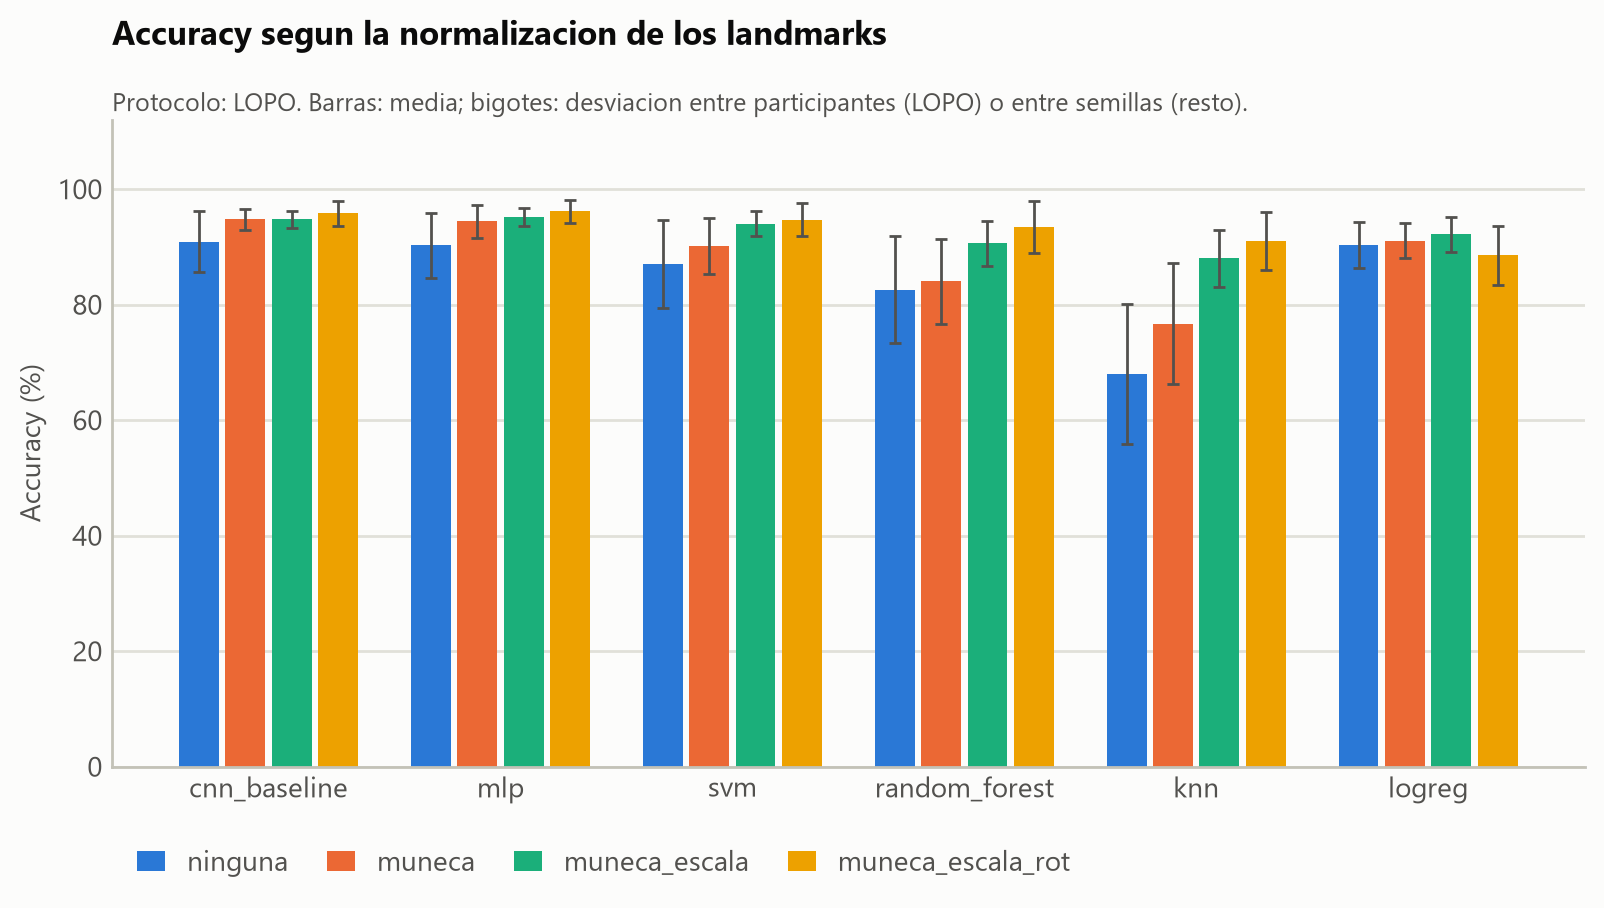
\includegraphics[width=0.92\linewidth]{normalizaciones_lopo}
\caption{Accuracy en LOPO de cada modelo con cada normalización.}
\end{figure}

Todos los modelos salvo la regresión logística mejoran al pasar de las coordenadas sin tocar a la normalización
completa, y la desviación entre personas se reduce a la mitad o menos: el modelo deja de depender de cómo graba cada uno. Los que más ganan son los que solo
miden distancias o umbrales sobre las coordenadas: $k$ vecinos sube 23 puntos y el random forest, 11. La regresión
logística, el único modelo lineal, es la excepción: rinde mejor sin el giro.

\subsection{Evaluar con personas nuevas}

\begin{table}[H]
\centering\small
\begin{tabular}{llccc}
\toprule
Modelo & Normalización & Temporal & LOPO & Temporal $-$ LOPO \\
\midrule
CNN del enunciado & muñeca + escala + giro & 94,3 & 95,8 & $-$1,5 \\
MLP & muñeca + escala + giro & 95,5 & 96,2 & $-$0,7 \\
SVM & muñeca + escala + giro & 92,9 & 94,7 & $-$1,8 \\
Random forest & muñeca + escala + giro & 92,6 & 93,4 & $-$0,9 \\
$k$ vecinos & muñeca + escala + giro & 90,4 & 91,0 & $-$0,6 \\
Regresión logística & muñeca + escala & 92,8 & 92,2 & +0,7 \\
\bottomrule
\end{tabular}
\caption{Misma configuración evaluada con el protocolo temporal y con LOPO (\%).}
\end{table}

Con los datos normalizados, el protocolo temporal y LOPO dan cifras parecidas (diferencia de 1,8 puntos como mucho).
El test temporal son los últimos 30 segundos de cada gesto, con posturas del final de la toma, así que tampoco es un
test fácil. Aun así, solo LOPO responde a la pregunta de la demo, y es el que usamos
para elegir.

\subsection{Experimentos de invarianza y aumentación}

\begin{table}[H]
\centering\small
\begin{tabular}{lcccc}
\toprule
\multirow{2}{*}{Experimento} & \multicolumn{2}{c}{MLP} & \multicolumn{2}{c}{CNN del enunciado} \\
\cmidrule(lr){2-3}\cmidrule(lr){4-5}
 & LOPO & Otra mano & LOPO & Otra mano \\
\midrule
Principal (sin aumentar) & 96,2 & 96,4 & 95,8 & 96,0 \\
Espejo por lateralidad & 95,9 & 95,9 & 95,9 & 95,9 \\
Aumentación (3 copias) & 96,1 & 96,2 & 95,8 & 95,9 \\
Aumentación con volteo & \mejor{96,5} & \mejor{96,6} & 96,2 & 96,2 \\
\bottomrule
\end{tabular}
\caption{Accuracy (\%) con la normalización completa. «Otra mano» es el test reflejado horizontalmente.}
\end{table}

Ningún modelo pierde acierto con la mano contraria, ni siquiera sin aumentación: con la normalización, una mano
izquierda y una derecha haciendo el mismo gesto ya se parecen lo suficiente. La aumentación con volteo es la que da el
mejor resultado y la que elegimos. El espejo por lateralidad no aporta, como cabía esperar de una etiqueta poco fiable.

\subsection{Errores por gesto}

\begin{figure}[H]
\centering
\begin{subfigure}{0.49\linewidth}
  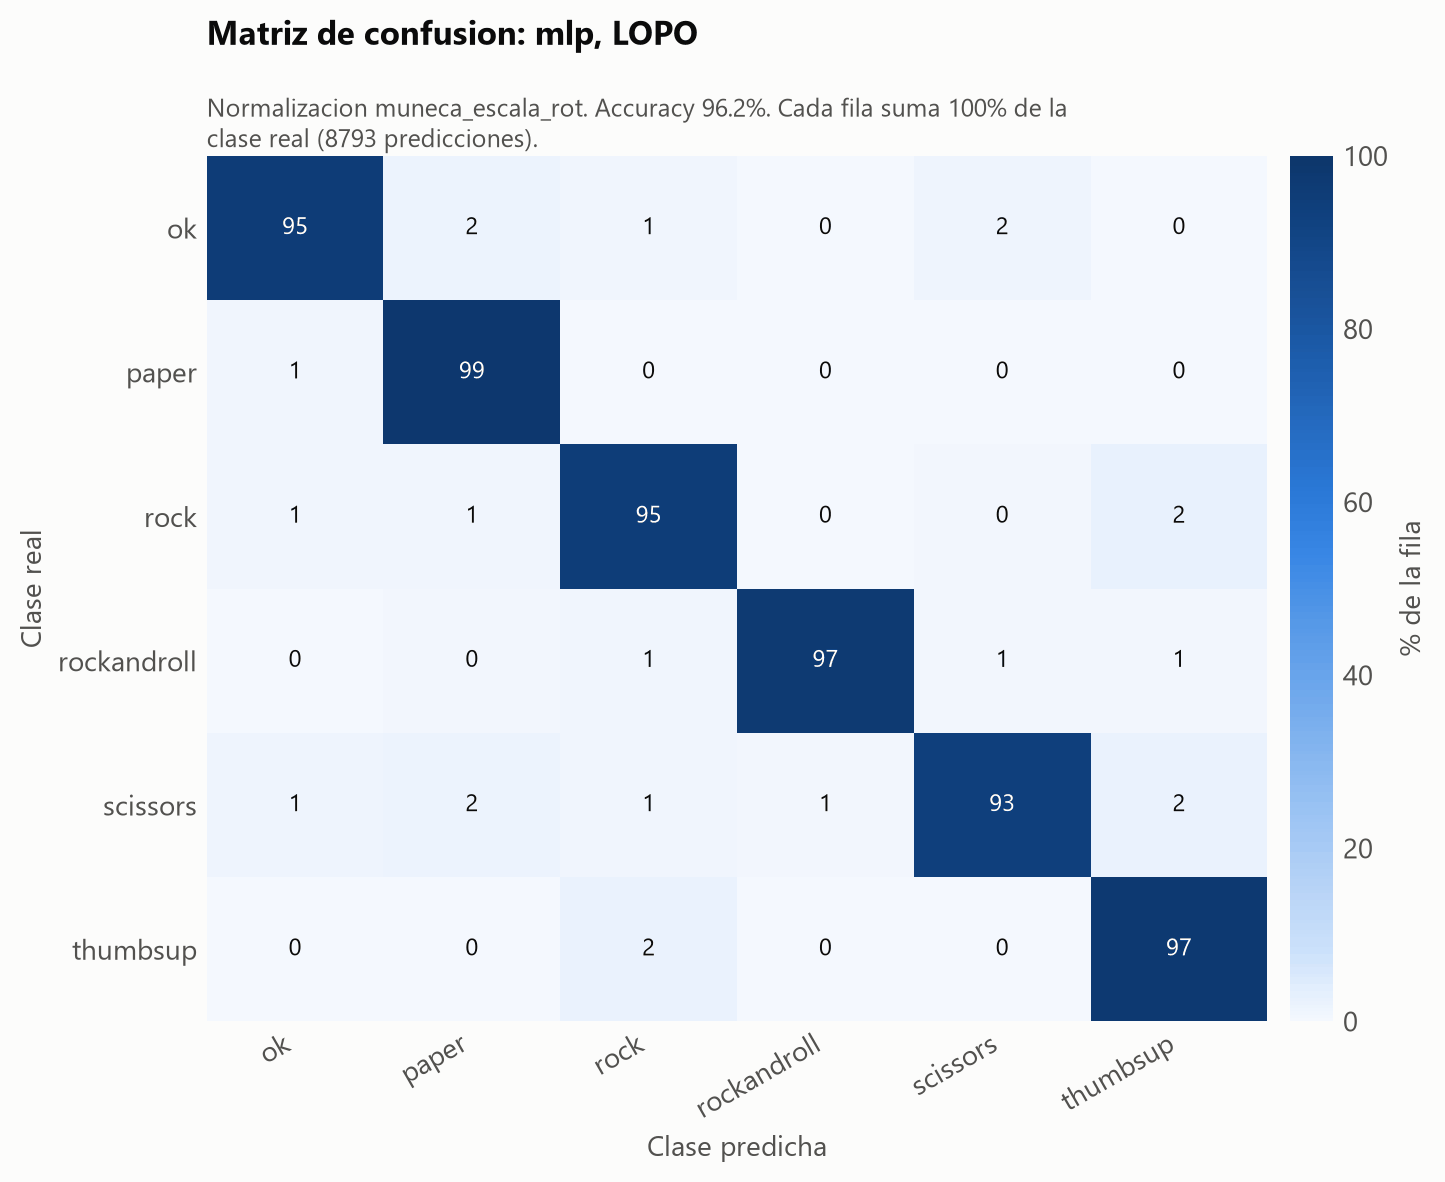
\includegraphics[width=\linewidth]{confusion_mlp_muneca_escala_rot_lopo}
  \caption{Matriz de confusión del MLP.}
\end{subfigure}\hfill
\begin{subfigure}{0.49\linewidth}
  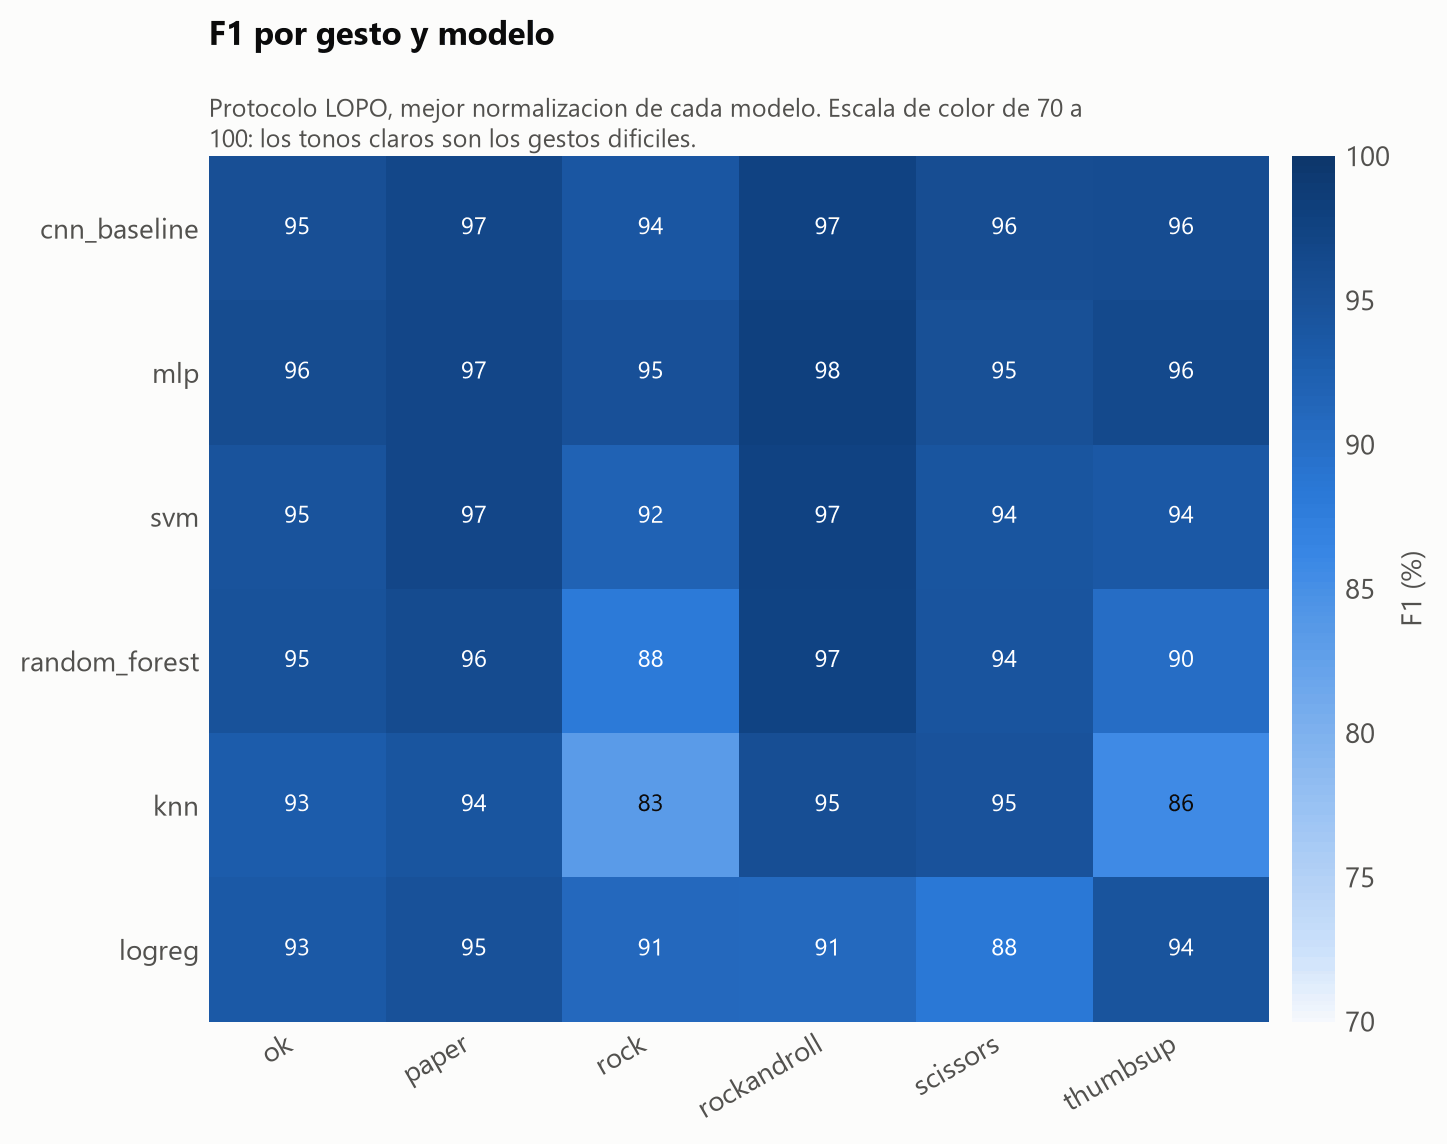
\includegraphics[width=\linewidth]{f1_por_clase_lopo}
  \caption{F1 por gesto y modelo.}
\end{subfigure}
\caption{Errores por gesto en LOPO con la normalización completa.}
\label{fig:confusion}
\end{figure}

El MLP no baja del \pct{93} de acierto en ningún gesto. Sus confusiones más frecuentes son \codigo{rock} tomado por
\codigo{thumbsup} (\pct{2,4} de los \codigo{rock}), \codigo{scissors} por \codigo{thumbsup} (\pct{2,0}),
\codigo{thumbsup} por \codigo{rock} (\pct{2,0}) y \codigo{ok} por \codigo{paper} (\pct{1,9}): los pares que la guía de
grabación ya señalaba. Los modelos más simples sufren en los mismos gestos: $k$ vecinos se queda en un F1 de 83 en
\codigo{rock} y de 86 en \codigo{thumbsup}.

\subsection{Acierto por persona}

\begin{table}[H]
\centering\small
\begin{tabular}{lccccc}
\toprule
Persona no vista & p1 & p2 & p3 & p4 & p5 \\
\midrule
MLP, normalización completa & 94,2 & 97,6 & 97,5 & 97,8 & 93,8 \\
CNN del enunciado, sin normalizar & 87,8 & 94,9 & 93,3 & 95,4 & 83,3 \\
\bottomrule
\end{tabular}
\caption{Accuracy (\%) con cada persona fuera del entrenamiento.}
\end{table}

p1 y p5 son las personas más difíciles: son las que grababan la mano más pequeña, es decir, más lejos de la cámara
(tabla~\ref{tab:dataset}). Son también las que más ganan con la normalización: p5 pasa del \pct{83,3} al \pct{93,8}.

\begin{figure}[H]
\centering
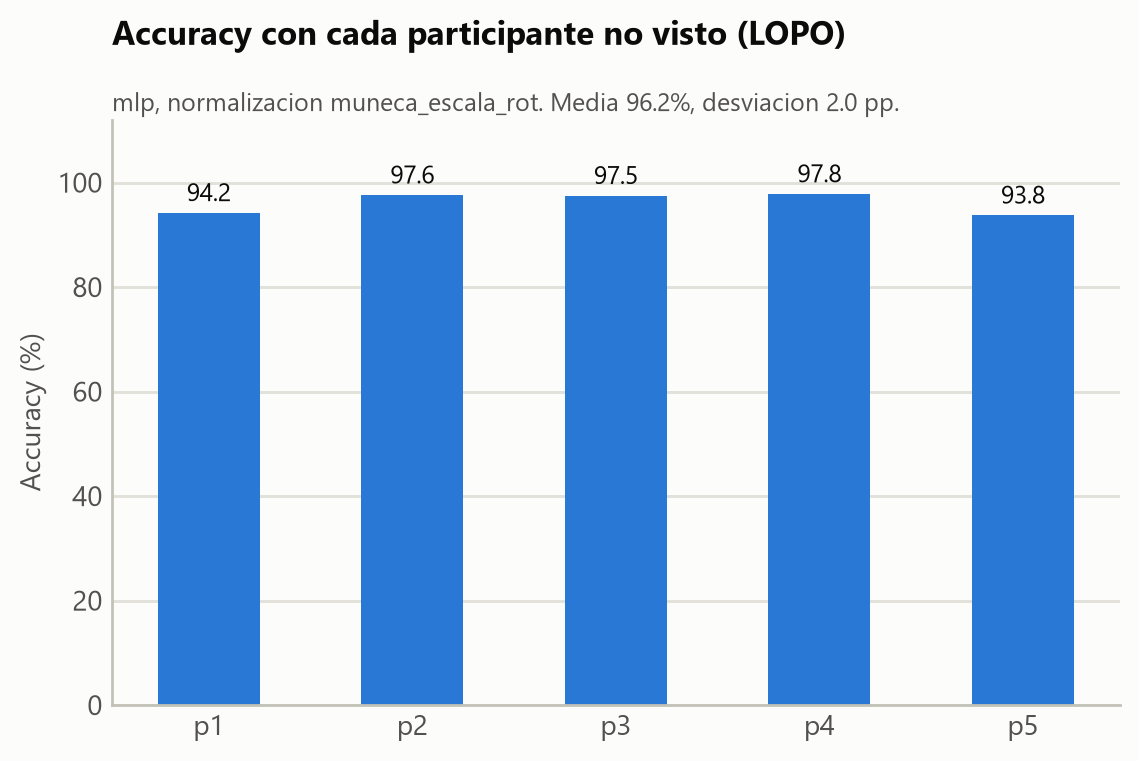
\includegraphics[width=0.7\linewidth]{participantes_mlp_muneca_escala_rot}
\caption{Accuracy del MLP con cada persona no vista.}
\end{figure}

\subsection{Coste computacional}
\label{sec:coste}

\begin{table}[H]
\centering\small
\begin{tabular}{lrrr}
\toprule
Modelo & Parámetros & Tamaño (KB) & Latencia (ms) \\
\midrule
MLP & \num{5030} & 86 & 0,84 \\
CNN del enunciado & \num{23126} & 303 & 1,23 \\
SVM & -- & 200 & 0,16 \\
Regresión logística & -- & 3 & 0,14 \\
Random forest & -- & \num{7546} & 6,26 \\
$k$ vecinos & -- & 304 & 10,32 \\
\midrule
Extractor de MediaPipe & -- & \num{7636} & 16,07 \\
\bottomrule
\end{tabular}
\caption{Coste por muestra con lote de 1 y un solo hilo de CPU, como en la demo (mediana de 300 a \num{1000} repeticiones).}
\end{table}

\begin{figure}[H]
\centering
\begin{subfigure}{0.49\linewidth}
  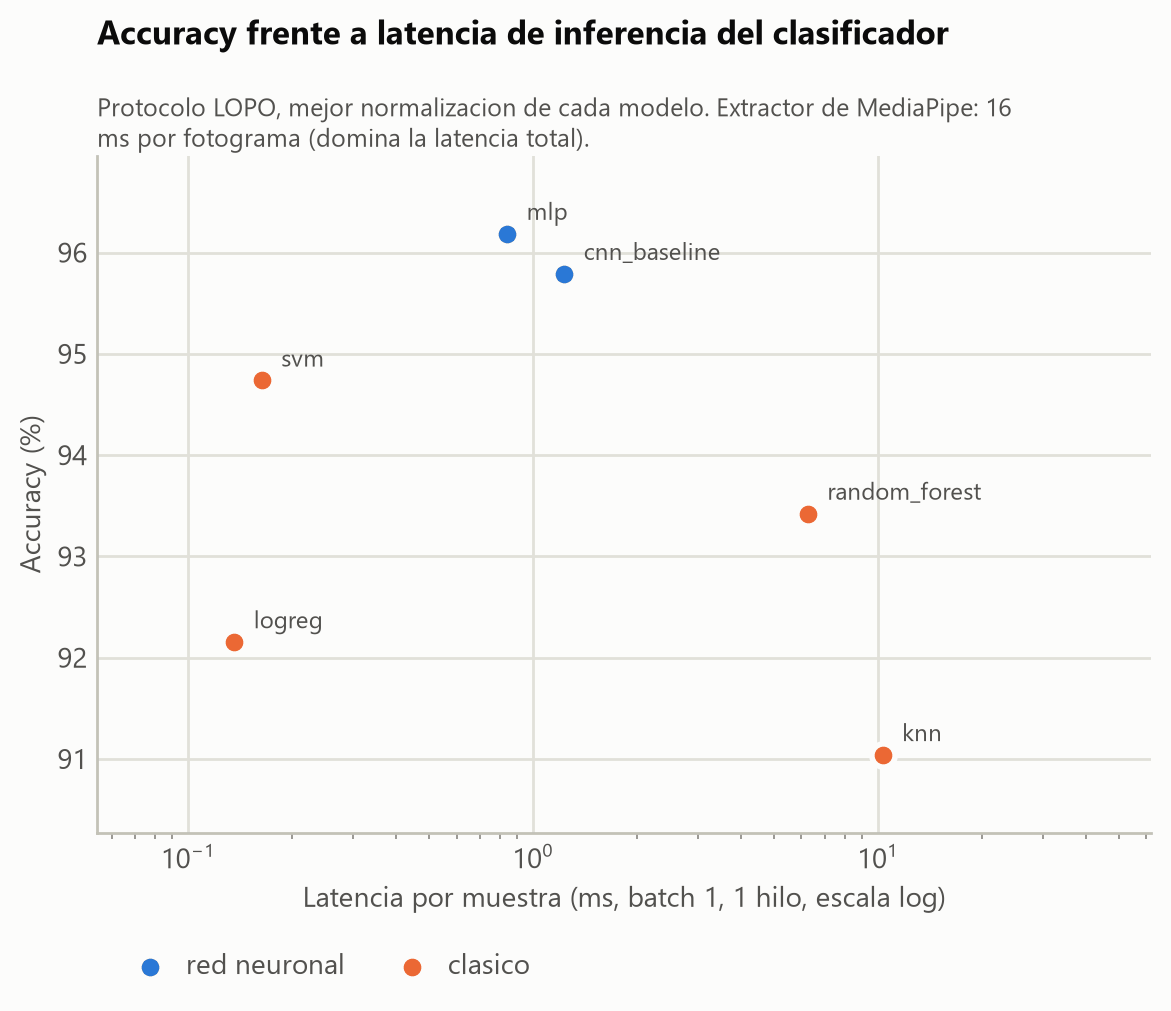
\includegraphics[width=\linewidth]{tradeoff_latencia}
\end{subfigure}\hfill
\begin{subfigure}{0.49\linewidth}
  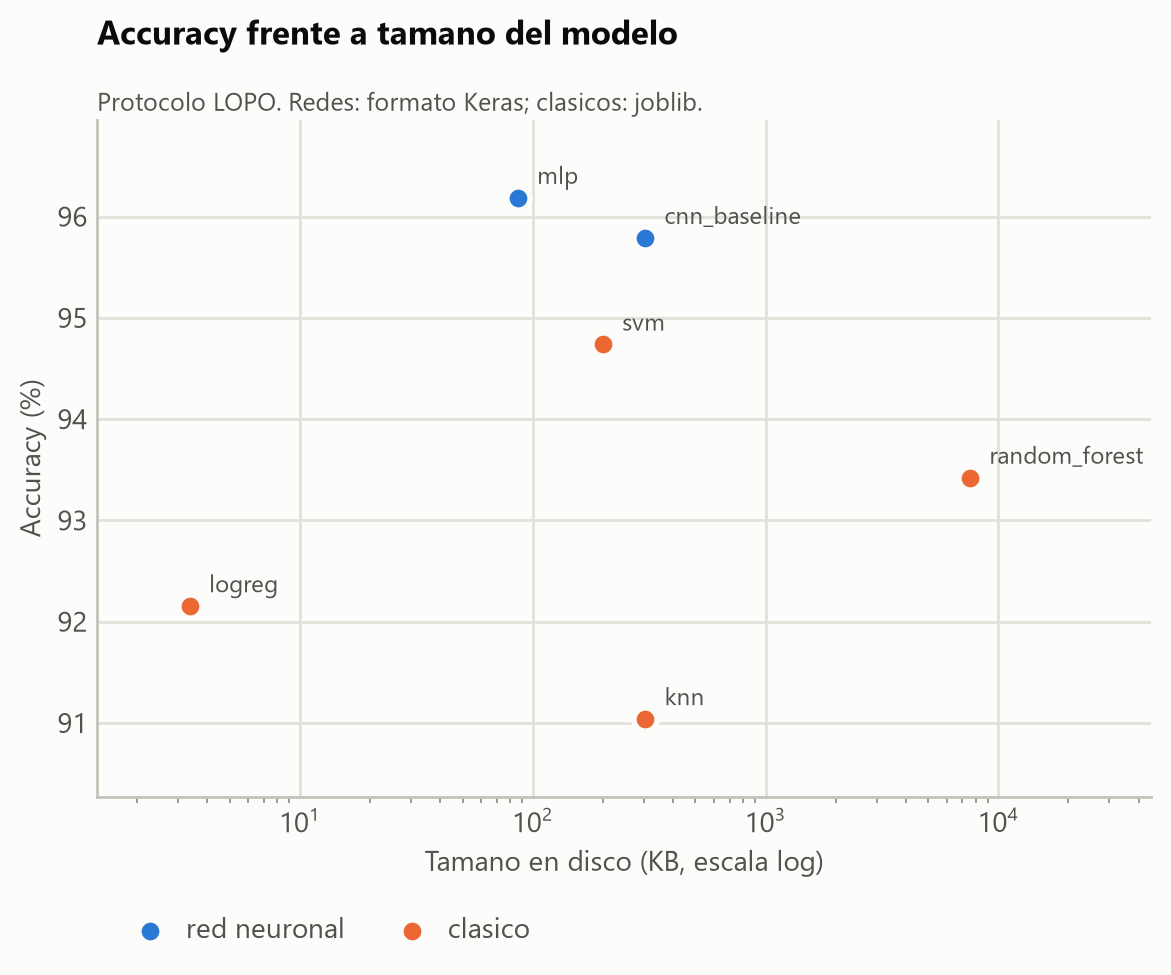
\includegraphics[width=\linewidth]{tradeoff_tamano}
\end{subfigure}
\caption{Acierto frente a latencia y frente a tamaño en disco.}
\end{figure}

La latencia la marca MediaPipe (16,1~ms), no el clasificador: con el MLP el techo teórico es de unos 59 fotogramas
por segundo. Entre los modelos, el MLP es el único que está a la vez en lo más alto en acierto y por debajo de 1~ms y
de 100~KB. El random forest ocupa 7,5~MB y $k$ vecinos guarda todo el entrenamiento y tarda más de 10~ms.

% ------------------------------------------------------------------ 7
\section{Modelo elegido y despliegue}

Elegimos el \textbf{MLP con la normalización completa y aumentación con volteo}: \pct{96,5} en LOPO y \pct{96,6} con
la otra mano. Frente a la CNN del enunciado acierta un poco más con cuatro veces menos parámetros, menos de un tercio
de tamaño y menos latencia. La convolución no aporta porque la entrada ya no es una imagen sino 42 coordenadas
normalizadas.

\begin{itemize}
  \item \textbf{Demo en tiempo real} (\codigo{demo/src/demo-gestures-PIDS.py}): abre la webcam, dibuja los puntos y
        muestra el gesto y la orden del tanque.
  \item \textbf{En el navegador}: los pesos se exportan a JSON y el portal web ejecuta MediaPipe para web y el MLP en
        TypeScript, sin servidor. Con 24 muestras reales del dataset, las probabilidades coinciden con las de Python a
        5 decimales.
  \item \textbf{Integración con la plataforma}: a la plataforma de datos solo llega el nombre del gesto y su confianza,
        nunca la imagen ni los puntos de la mano. Encaja con el escenario E3 de privacidad de las fases 2 y 3.
\end{itemize}

% ------------------------------------------------------------------ 8
\section{Análisis sin etiquetas}

Como análisis complementario comprobamos si los gestos se separan solos, sin dar ninguna etiqueta al algoritmo.
Agrupamos las \num{2931} manos con $k$-means y con el método de Ward y las proyectamos en dos dimensiones con t-SNE.
El acuerdo entre grupos y etiquetas se mide con el índice de Rand ajustado (ARI: 0 equivale al azar y 1 a grupos
idénticos). La tercera representación añade a la normalización completa el espejo por lateralidad.

\begin{table}[H]
\centering\small
\begin{tabular}{lcccc}
\toprule
Representación & ARI con el gesto & Manos en el grupo de su gesto & ARI con la persona \\
\midrule
Sin normalizar & 0,05 & \pct{27,8} & 0,05 \\
Normalizada & 0,22 & \pct{37,6} & 0,01 \\
Normalizada + espejo & \mejor{0,36} & \mejor{\pct{49,9}} & 0,03 \\
\bottomrule
\end{tabular}
\caption{$k$-means con 6 grupos (uno por gesto) y con 5 (uno por persona).}
\end{table}

\begin{figure}[H]
\centering
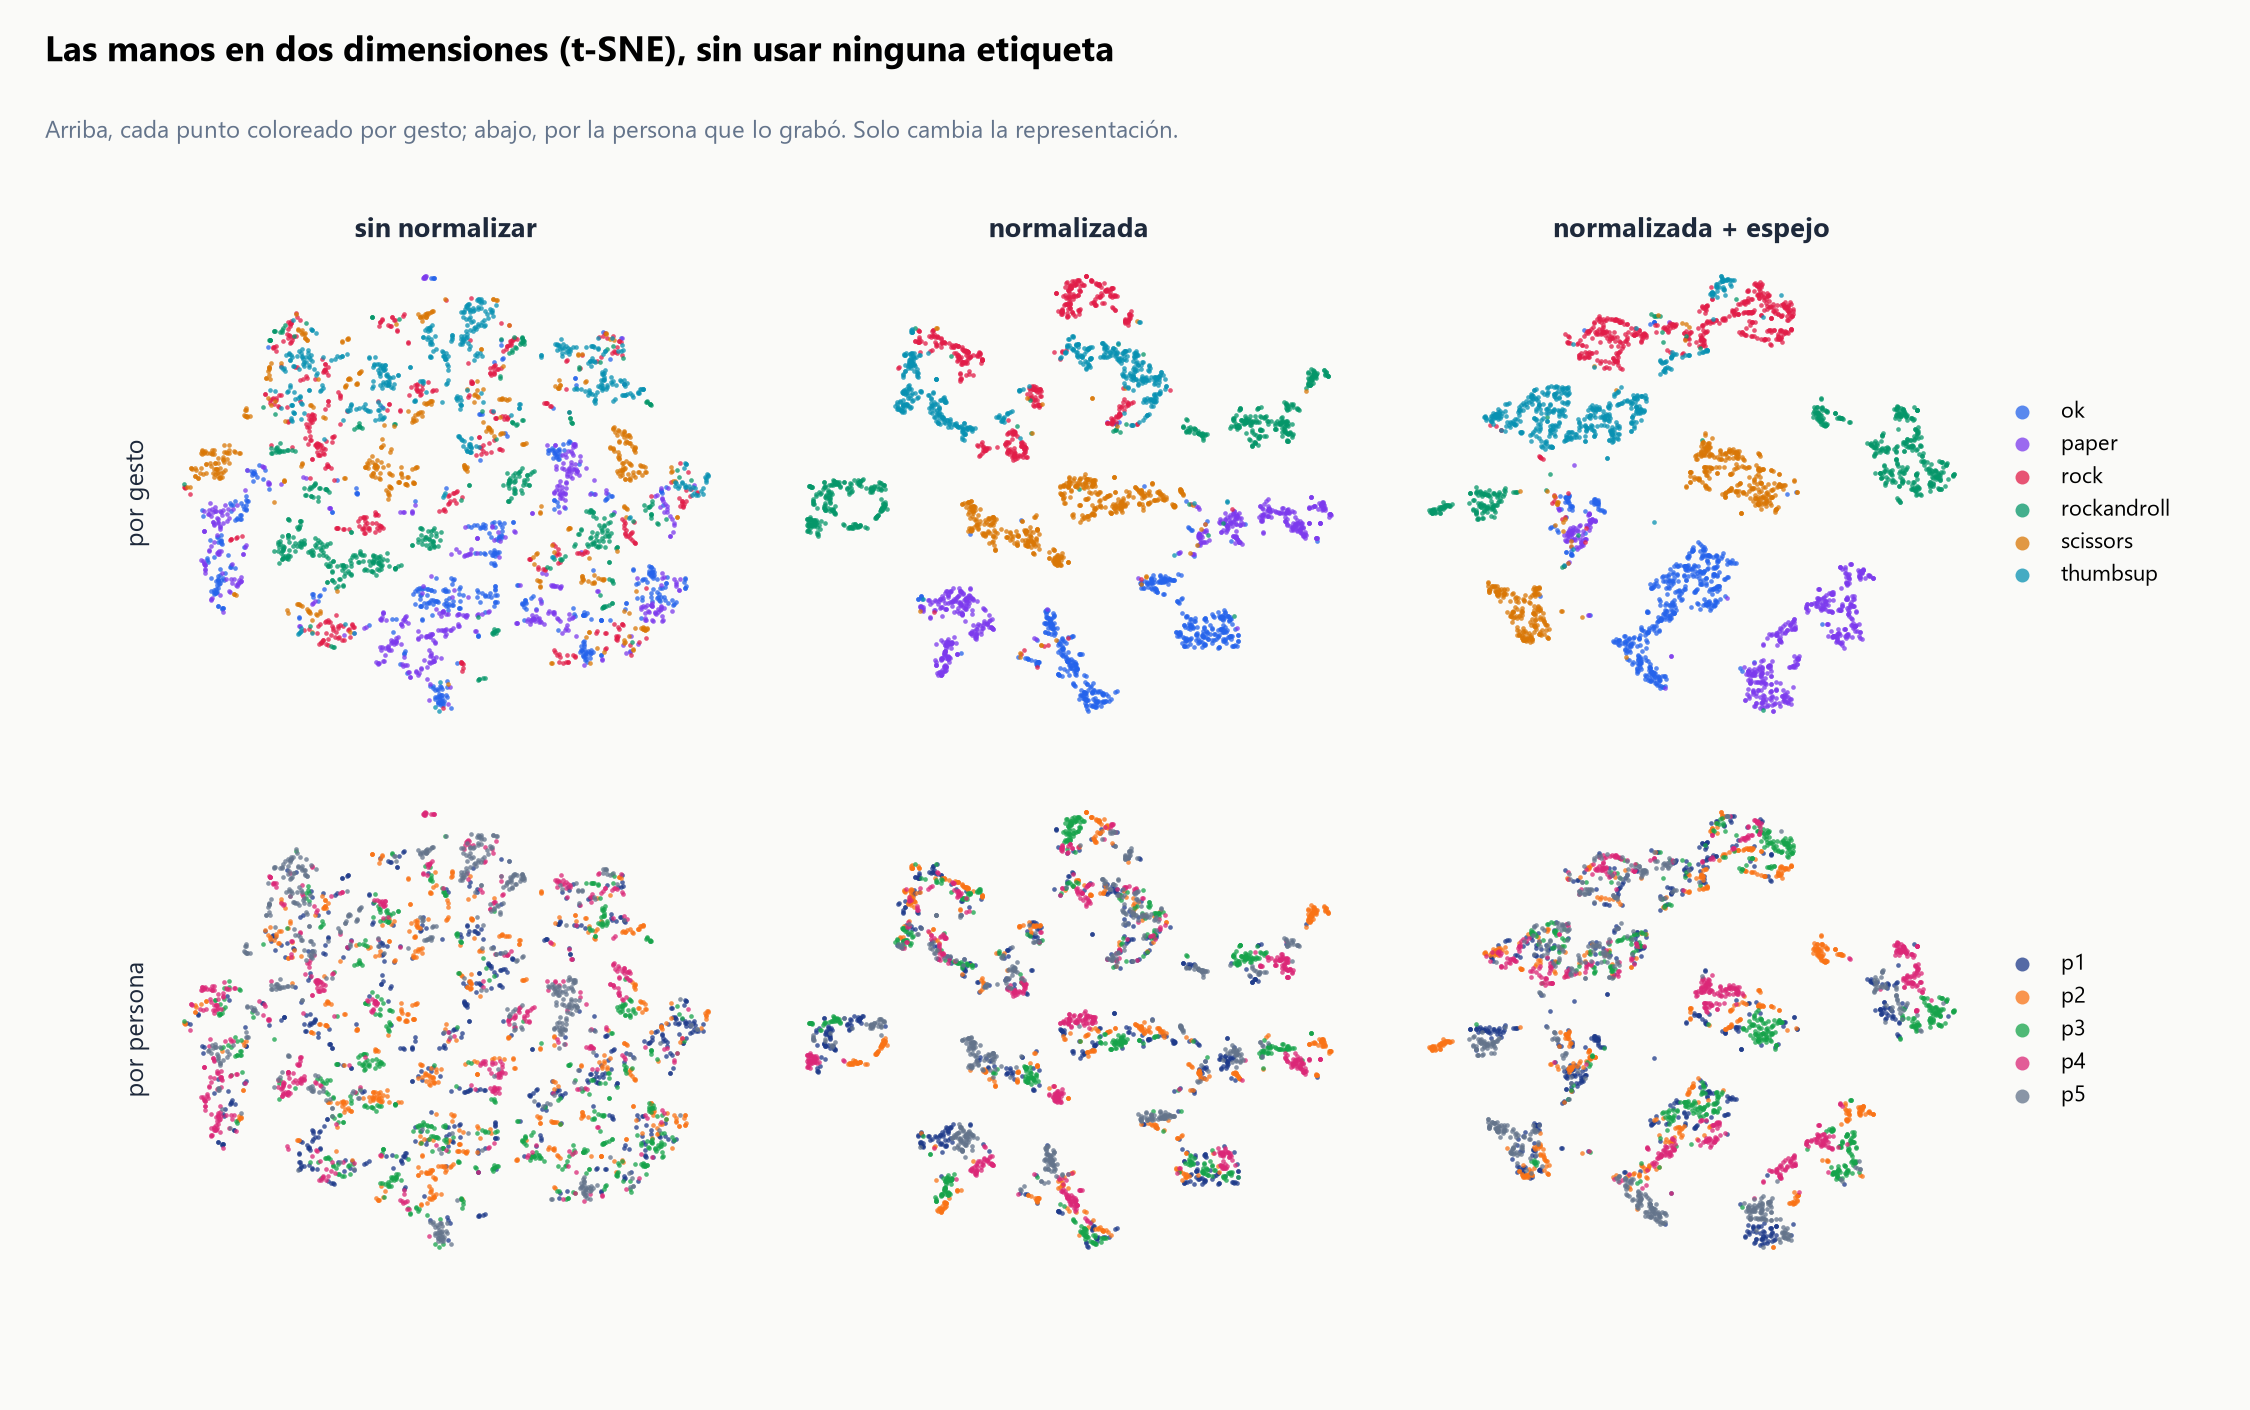
\includegraphics[width=\linewidth]{tsne_gesto_persona}
\caption{Proyección t-SNE de las manos con cada representación, coloreada por gesto (arriba) y por persona (abajo).}
\label{fig:tsne}
\end{figure}

\begin{itemize}
  \item \textbf{La normalización hace aparecer los gestos}: sin normalizar todo está mezclado; normalizado aparecen
        islas de un solo gesto, y el acuerdo con los gestos se multiplica por siete.
  \item \textbf{Las personas no se agrupan} en ninguna representación (ARI entre 0,01 y 0,05): lo que distingue a las
        manos es el gesto, no quién lo hace.
  \item \textbf{Cada gesto tiene variantes}: con 6 grupos solo la mitad de las manos cae en el de su gesto (por
        ejemplo, \codigo{ok} y \codigo{paper} acaban juntos), pero con más grupos la cifra sube deprisa: \pct{83} con
        12 y \pct{91} con 20, lo mismo que $k$ vecinos supervisado (figura~\ref{fig:subgrupos}).
\end{itemize}

\begin{figure}[H]
\centering
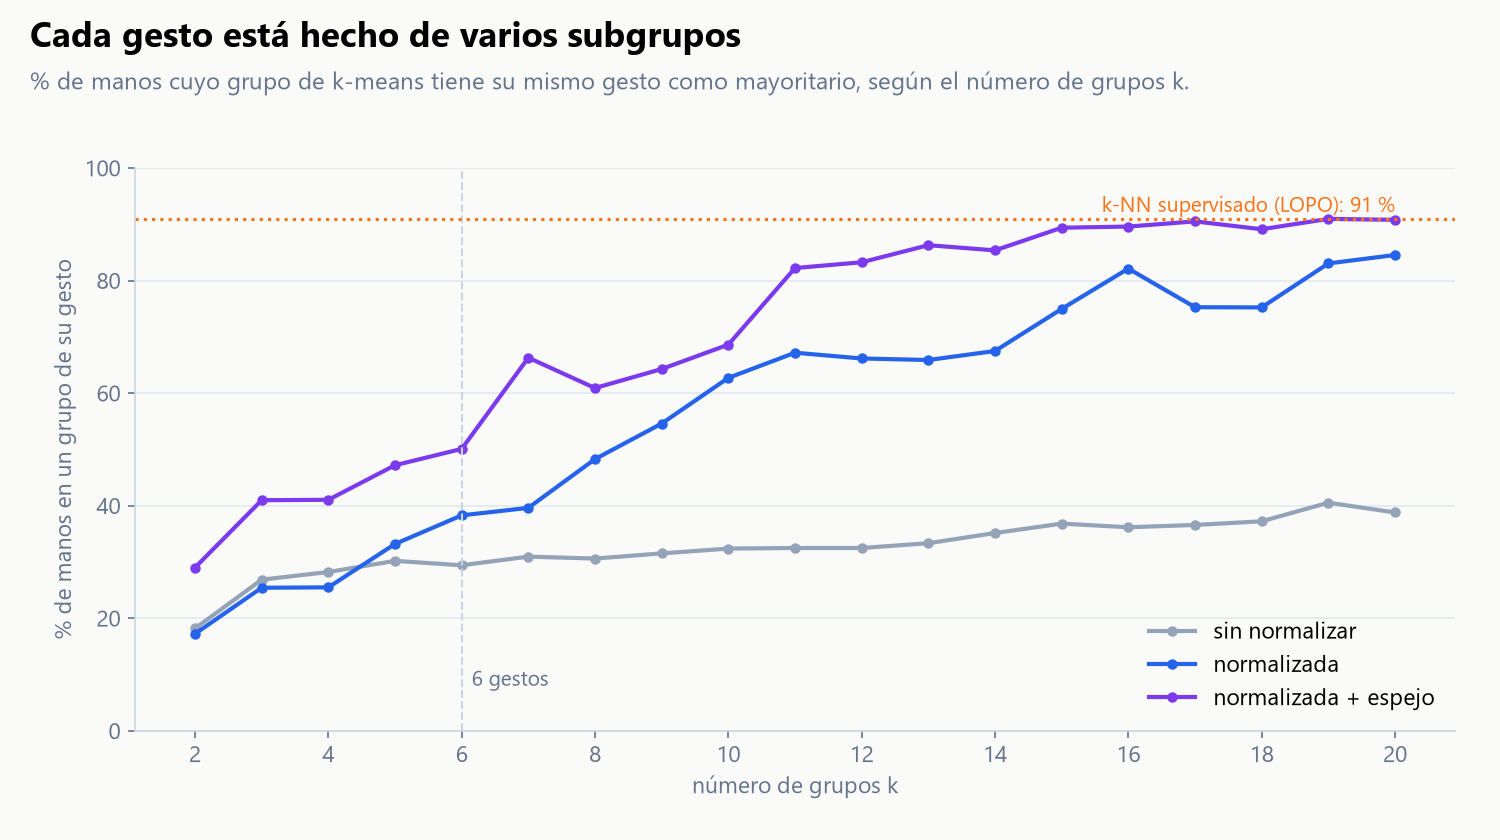
\includegraphics[width=0.85\linewidth]{subgrupos_por_k}
\caption{Porcentaje de manos cuyo grupo de $k$-means tiene su gesto como mayoritario, según el número de grupos.}
\label{fig:subgrupos}
\end{figure}

La conclusión es que los gestos tienen estructura propia, pero hace falta un clasificador supervisado para unir las
variantes de cada uno.

% ------------------------------------------------------------------ 9
\section{Limitaciones}

\begin{itemize}
  \item \textbf{Cinco personas y pocas condiciones}: las tomas se grabaron en dos días y en entornos parecidos. Con más
        personas, luces y cámaras la estimación de LOPO sería más fiable; su desviación entre personas
        ($\pm$2 puntos) indica cuánto puede variar con alguien nuevo.
  \item \textbf{Sin clase de «ningún gesto»} en la evaluación: el clasificador siempre elige uno de los seis.
  \item \textbf{Solo coordenadas 2D}: no usamos la profundidad estimada por MediaPipe.
  \item \textbf{Sin TensorFlow Lite}: no se pudo generar porque la política de seguridad del portátil bloquea
        TensorFlow. Para el navegador lo resolvimos exportando el MLP a JSON.
\end{itemize}

% ------------------------------------------------------------------ 10
\section{Conclusiones}

\begin{enumerate}
  \item \textbf{La representación importa más que el modelo}: con los mismos datos, normalizar sube todos los modelos
        y reduce a la mitad la diferencia entre personas.
  \item \textbf{Medir con personas nuevas cambia las conclusiones}: LOPO es la única cifra que dice qué pasará en una
        demostración, y con ella la diferencia entre la CNN y el MLP es pequeña.
  \item \textbf{Lo sencillo gana}: un MLP de 86~KB acierta tanto o más que la CNN, corre en menos de 1~ms y se ejecuta
        en el navegador, lo que permitió integrar la fase 1 en el portal sin enviar ninguna imagen.
\end{enumerate}

% ------------------------------------------------------------------ anexo
\clearpage
\appendix
\section{Reproducibilidad}

Todo el código está en la carpeta \codigo{parte1\_gestos/} del repositorio:

\begin{table}[H]
\centering\small
\begin{tabularx}{\linewidth}{lX}
\toprule
Ruta & Contenido \\
\midrule
\codigo{kit\_grabacion/} & Grabador del dataset y su guía \\
\codigo{entrenamiento/} & Preprocesado, rejilla de experimentos, evaluación y exportación (paquete \codigo{hgr}, con tests) \\
\codigo{entrenamiento/clustering.py} & Análisis sin etiquetas de la sección 8 \\
\codigo{datos\_generados/} & Puntos de la mano de las \num{3000} imágenes \\
\codigo{resultados/} & Informe, tablas y figuras de cada experimento, comparativa y clustering \\
\codigo{modelos/} & MLP y CNN exportados \\
\codigo{demo/} & Demo en tiempo real y notebooks \\
\bottomrule
\end{tabularx}
\end{table}

Con el dataset descomprimido y \codigo{PIDS\_DATOS} apuntando a él, se reproduce con:

\begin{verbatim}
python parte1_gestos\descargar_modelos.py
python parte1_gestos\entrenamiento\preprocesar.py
python parte1_gestos\entrenamiento\entrenar_todo.py
python parte1_gestos\entrenamiento\clustering.py
\end{verbatim}

Versiones: Python 3.12, MediaPipe 0.10.35, Keras 3.15.1 (sobre PyTorch), scikit-learn 1.9.0.

\end{document}
